\documentclass{article}[12pt]

% GRAPHICS
\usepackage{float}
\usepackage{graphicx}
\usepackage{subcaption}

% HYPERLINKS
\usepackage{hyperref}

% DOCUMENT PADDING AND MARGINS
\usepackage{titlesec}
\usepackage[margin=1.5in]{geometry}
\setlength{\parskip}{\baselineskip}%
\setlength{\parindent}{0pt}
\titlespacing*{\section}{0pt}{2ex}{0ex}
\titlespacing*{\subsection}{0pt}{1ex}{-2ex}
\titlespacing*{\subsubsection}{0pt}{2ex}{-2ex}

%COMMENTING
\usepackage{comment}


\begin{document}

% TITLE
\title{Autonomous Quadrotor Landing on a Moving Platform}
\author{Stan Brown \& Chris Choi}
\date{}
\maketitle



\section*{Introduction}
Our goal is to autonomously land a quadrotor onto a moving platform, the main 
significance of this work is to disgard GPS and perform autonomous precision 
landing using low cost sensors, such as sonar and vision.

In this interim-report we will discuss our progress, and any preliminary 
results we may have. So far we have spent a considerable amount of effort 
getting different components of the project working. In this report we will be 
discussing changes, progress in both hardware and software aspects of the 
project and remaining project schedule.



\section*{Changes in Direction or Project Scope}

Due to time constraints, we will be forgoing our idea of using gimbal cameras 
for this project. We initially had hoped we would be using the gimbal camera 
to locate the landing target from afar and approach the target. 

Since we are omitting gimbal cameras, we will be assuming that the 
quadrotor will be directly above the moving landing target as its intial 
conditions, and that is where our autonomous system will be to start its 
autonoums precision landing.



\section*{Project Progress}
\subsection*{Hardware}
\subsubsection*{Quadrotor Setup}
For the hardware, we have chosen to reuse equipment that is readily available 
to us in the Wave Lab. For the quadrotor we have been using the DJI F450 
quadrotor frame, Emax 2213-935KV motors with complimentary 1045R propellers, 
Thunder Power lipo 11.1V 4200mah battery, DJI E310 420S 20A electronic speed 
controller and Pixhawk v2.4 as our flight controller. At current our quadrotor 
flies reasonably well with some \textit{minor} setbacks, mainly due to the 
instability of the firmware, and lack of good documentation for the firmware 
and software packages. Our problems thus far with the quadcopter are mostly 
software based.

\begin{figure}[H]
	\centering
	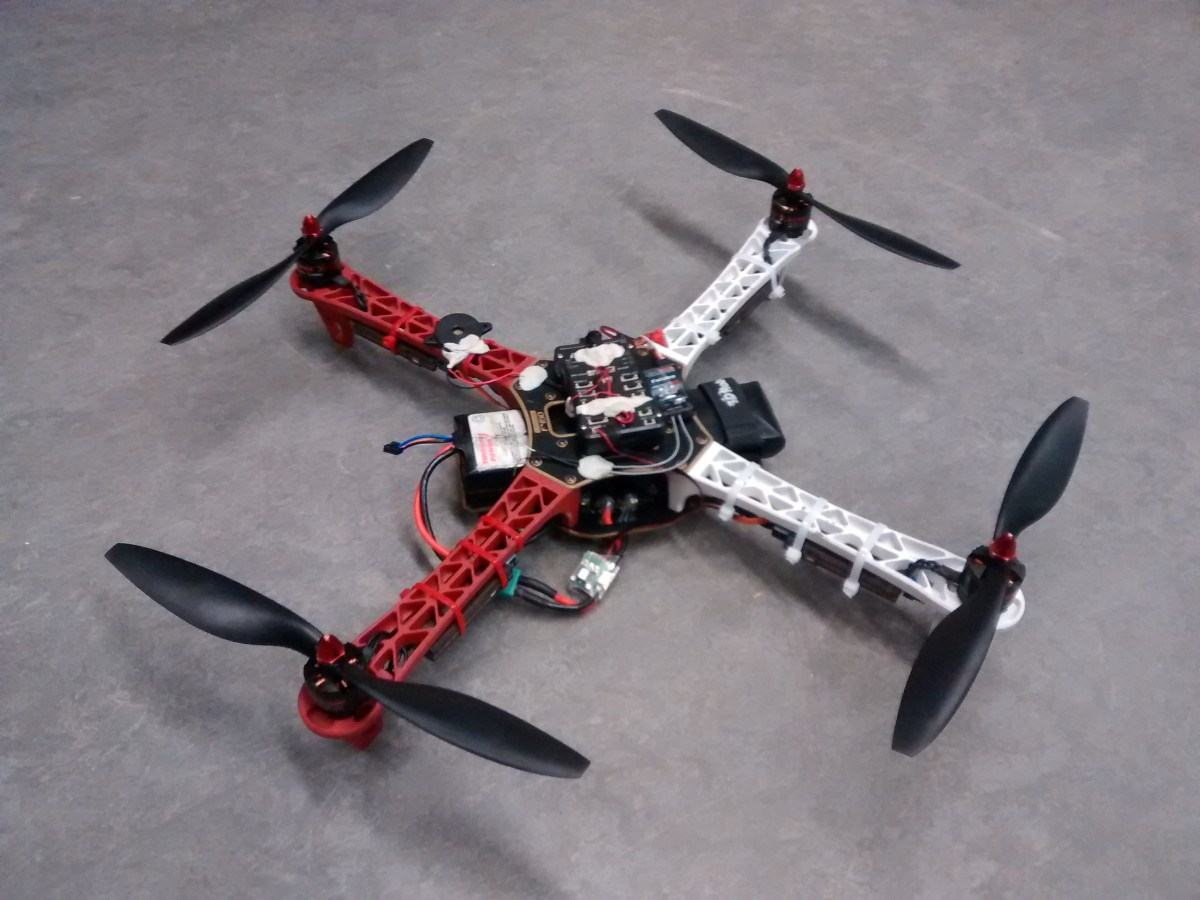
\includegraphics[width=0.6\textwidth]{images/quadrotor.jpg}
	\caption{DJI F450 with Pixhawk v1.5}
\end{figure}

\subsubsection*{Onboard Autonomous Control System}
In terms of onboard autonoumos control, we have decided to use the Odriod 
XU4 due to its size and processing power available, and a Logitech C270 HD 
webcam as our vision sensor. One problem we may face very soon is the narrow 
field of view and relatively low frame rate (25Hz) the logitech webcam has. We 
will be keeping our options open, and plan on replacing the logitech webcam 
with a Ximia xiQ USB3 camera with a wide angle lens in the near 
future.



\subsection*{Software}
\subsubsection*{Pixhawk Firmware}
As mentioned in the hardware section, we have had numerous issues with 
regards to using the software suite for the Pixhawk Flight Controller, 
as well as the PX4 firmware itself. There are many instances where we could not 
explain the instability of the quadrotor during flight, many of which lead to 
costly crashes, but we believe through these experiences we have developed a 
procedure to lower the risk for such instances from happening often.

\subsubsection*{Odriod to Pixhawk Communication}
For our autonomous system to control the quadrotor directly, the Odriod has to 
be able to communicate with the Pixhawk, this is where \verb|mavros| (ROS 
package) comes into play. Mavlink is a popular UAV communication protocol 
between UAV and ground control softwares, \verb|mavros| creates a mavlink ROS 
node to enable developers to monitor and issue mavlink commands with ease. We 
have successfully used mavros to arm and disarm Pixhawk (tested), in the near 
future we should be able to send velocity/attitude commands to control the 
quadrotor.

\subsubsection*{Simulator}
Initially we have explored the possibility of using the combination of PX4's 
Software in the Loop Simulation (SITL) and Gazebo 6 as our simulation 
environment for our project, however we found the combination of install 
instructions changing at a fast pace, and the documentation not up to date to 
be a major concern for us. We have therefore decided to fallback on developing 
the estimation and control loop in Matlab.

\subsubsection*{AprilTag}
\begin{figure}[H]
	\centering
	\begin{subfigure}[b]{0.45\linewidth}
		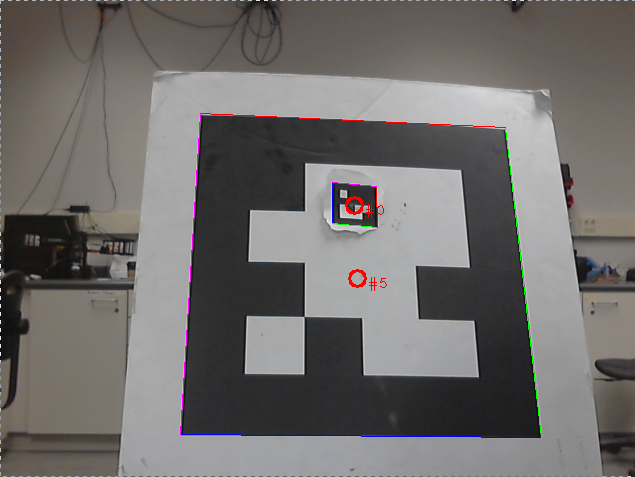
\includegraphics[width=\textwidth]{images/apriltags_1.png}
		\caption{2 Apriltags Detected}
	\end{subfigure}
	\begin{subfigure}[b]{0.45\linewidth}
		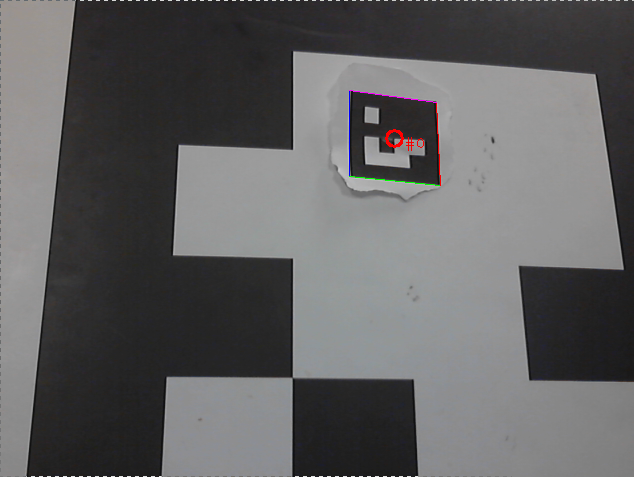
\includegraphics[width=\textwidth]{images/apriltags_3.png}
		\caption{1 Apriltag Detected }
	\end{subfigure}
	\caption{Apriltag Inception - To mitigate the FOV problem}
	\label{fig:apriltag}
\end{figure}

On the landing target from we have successfully calibrated the logitech webcam 
and used the Apriltag library to obtain a pose estimate, and have manually 
verified the estimates are accurate, for distance the error is $\pm 1$cm. We 
have also successfully implemented the ability to identify two different 
apriltags of different sizes (see Fig~\ref{fig:apriltag}), pose estimates from 
both apriltags are equal.

Next is to workout how to transform the measurements from the pose estimates of 
the apriltags in relation to the quadrotor's body frame.



\section*{Schedule}

\begin{itemize}
	\vspace{-0.2cm}
	\setlength{\itemsep}{5pt}
	\setlength{\parskip}{0pt}
	\setlength{\parsep}{0pt}
	
	\item{\textbf{6th March}: Implement and show in simulation that we can land 
	a quadrotor successfully on to a moving platform}
	\item{\textbf{13th March}: Perform Autonomous Flying Outdoors and Implement 
	Control code for the Huskey}
	\item{\textbf{21st March}: Perform Autonomous Flying Indoors}
	\item{\textbf{28th March}: Attempt to Autonomous Land the Quadrotor Indoors}
\end{itemize}






\bibliography{proposal}{}
\bibliographystyle{ieeetr}

\end{document}
